% !TEX root = main.tex

\section{2D vortex-in-cell problem}~\label{App_2D}
\subsection{Description of the method}


In this section, we apply the Vortex Method in a two-dimensional scenario, as outlined by Cottet et al. \cite{cottet_vortex_2000}. The Vortex Method is a Lagrangian approach utilizing a particle ensemble to discretize the vorticity field, allowing for the solution of the Navier-Stokes equation for viscous incompressible flow. The method is grounded in the vorticity-velocity formulation of the Euler equation, where $\bm \omega = \nabla \times \bm{v}$ satisfies

\[
	\begin{aligned}
		\frac{\partial \bm \omega}{\partial t} + (\bm{v} \cdot \nabla) \bm \omega - \nu \Delta \bm \omega & = 0, \\
		\nabla \cdot \bm v                                                                                & = 0,
	\end{aligned}
\]where $\omega$ denotes vorticity, $\bm{v}$ represents velocity, and $\nu$ stands for viscosity.

In the context of 2D flow, vorticity is perpendicular to the flow plane, forming a scalar field denoted as $\omega$. In Cartesian coordinates, it is expressed as $\omega = \frac{\partial v_y}{\partial x} - \frac{\partial v_x}{\partial y}$.

The vorticity field is discretized using a collection of discrete vortices, each characterized by a position $\bm z_p$, an associated kernel $\phi_\varepsilon$, and a circulation $\Gamma_p$. For all points $\bm z$ within the domain $\Omega$, the vorticity is expressed as

\begin{equation*}
	\omega(\bm z) = \sum_{i=1}^{N_p} \Gamma_p \phi_\varepsilon(\bm z - \bm z_p).
\end{equation*}

To address the Navier-Stokes equation, we employ a viscous splitting scheme, following the methodology outlined in \cite{cottet_1990}, acknowledging the predominance of the convection term over viscosity. We use the Vortex-In-Cell algorithm \cite{christiansen_1973, birdsall_1969}, coupled with an FFT solver to cumpute the advection velocity. The subsequent steps involve assigning particle vorticity values to the grid using a particle-to-grid formula, computing the velocity field by solving the Poisson equation on the grid verified by the stream function. Finally, the velocity is interpolated back onto the particles using the grid-to-particles formula. A Runge-Kutta 3 time-stepping scheme is employed to update the particle positions through a time integration scheme. The final phase involves solving the heat equation and update the particles intensities thanks to the PSE method previously described in Section~\ref{App_1D}.

\subsection{Lamb-Chaplygin dipole and simulation parameters}

We define the reference as the advection of the Lamb-Chaplygin dipole inside a close domain with stress-free walls. Lamb-Chaplygin dipole is a popular choice for numerical studies \cite{orlandi_vortex_1990}. The model represents a specific steady, inviscid dipolar vortex flow and offers a non-trivial solution to the two-dimensional Euler equations. The dipole is characterized by a translation velocity $U$, a mean position $\bm{z}_0$, a radius $R$, and an orientation $\alpha$.

The dipole vorticity field $\omega$ could be expressed as

\begin{equation*}
	\omega(r) = \begin{cases}
		\frac{-2 k U J_1(kr)}{J_0(kR)} \sin \alpha \quad & \text{for} \quad  r < R, \\
		0 \quad                                          & \text{otherwise},
	\end{cases}
\end{equation*}where $(r, \alpha)$ represent the polar coordinates in the dipole reference frame. Here, $J_0$ and $J_1$ denote the zeroth and first order Bessel functions of the first kind, respectively, and $k$ is determined such that $kR$ corresponds to the first non-trivial zero of the first Bessel function.  The dipole vorticity field is depicted in Figure \ref{fig:lamb_dipole}.

\begin{figure}[ht]
	\centering
	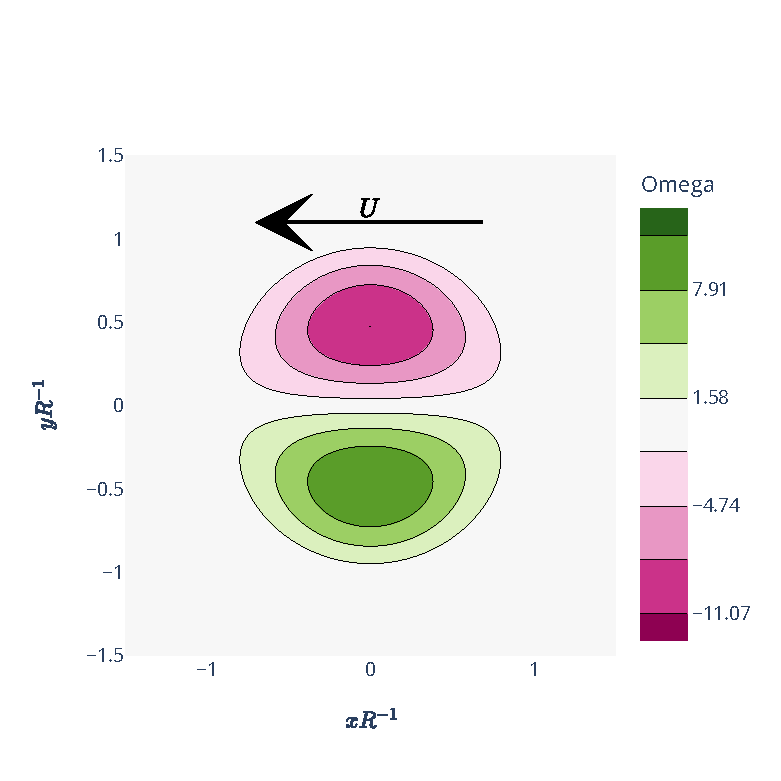
\includegraphics[width=0.6\linewidth]{images/app2d/lamb.pdf}
	\caption{The Lamb-Chaplygin dipole vorticity field on a normalize space.}
	\label{fig:lamb_dipole}
\end{figure}

The dipole is positioned at the center of a box with dimensions $[0, \pi] \times [0, \pi]$, featuring an orientation of $\frac{7\pi}{8}$ rad., a radius of $0.5$ meters, and a velocity $U$ of $0.25 \text{ m.s}^{-1}$. The complete reference setting is listed in Table \ref{tab:ref}.

The boundary box features stress-free walls, meaning fluid cannot pass through them. The velocity perpendicular to the walls is zero, while tangential velocity remains undetermined. When a vortex, such as a dipole, reaches this boundary, it walks along the wall, sensing its reflection and interacting with it.

Because this problem does not have an explicit solution on a closed domain, we simulate the ground truth with the vortex method for a fined discretization and fixed set of parameters described also in Table \ref{tab:ref}. The trajectory of the ground truth is illustrate in the Figure \ref{fig:ref_trajectory} on a regularly spaced grid.

\begin{figure}[htbp]
	\begin{subfigure}{0.32\textwidth}
		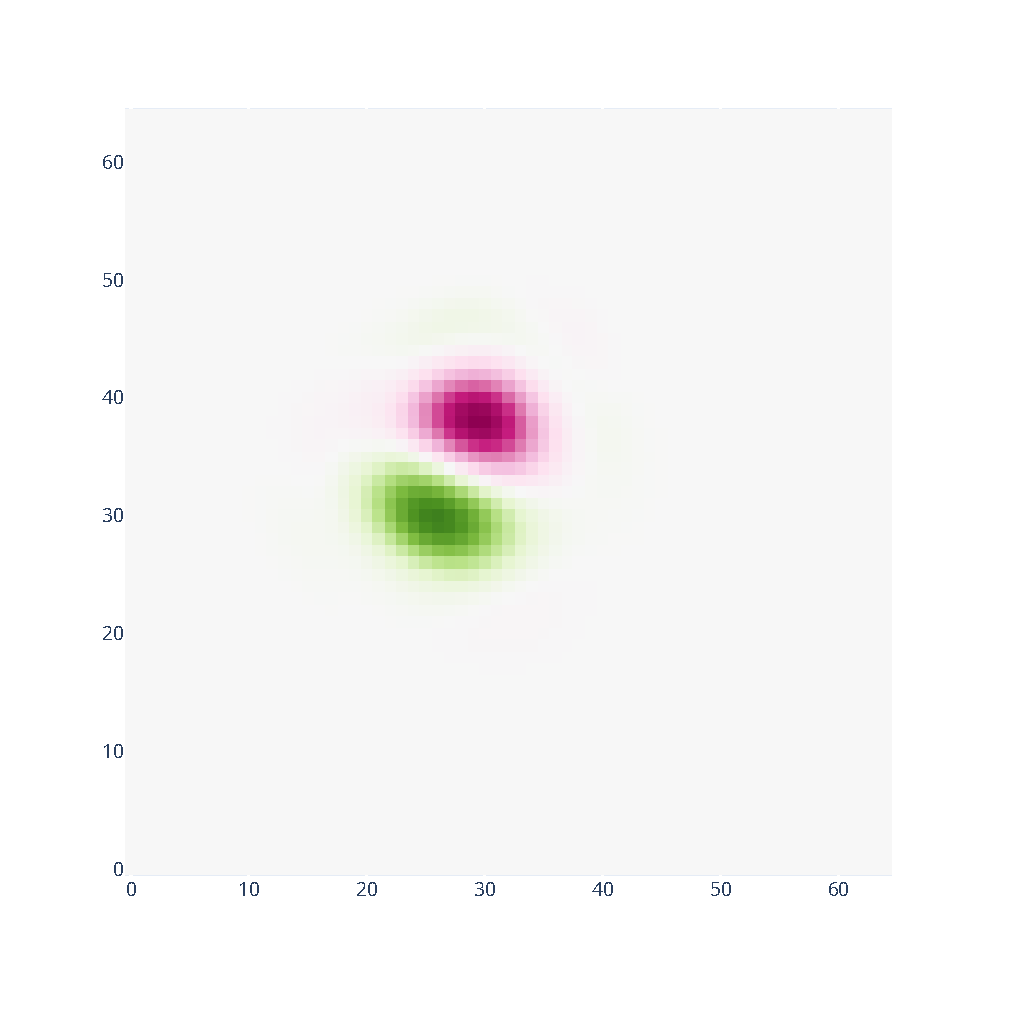
\includegraphics[width=\linewidth]{images/app2d/best_estimate_2.pdf}
	\end{subfigure}
	\hfill
	\begin{subfigure}{0.32\textwidth}
		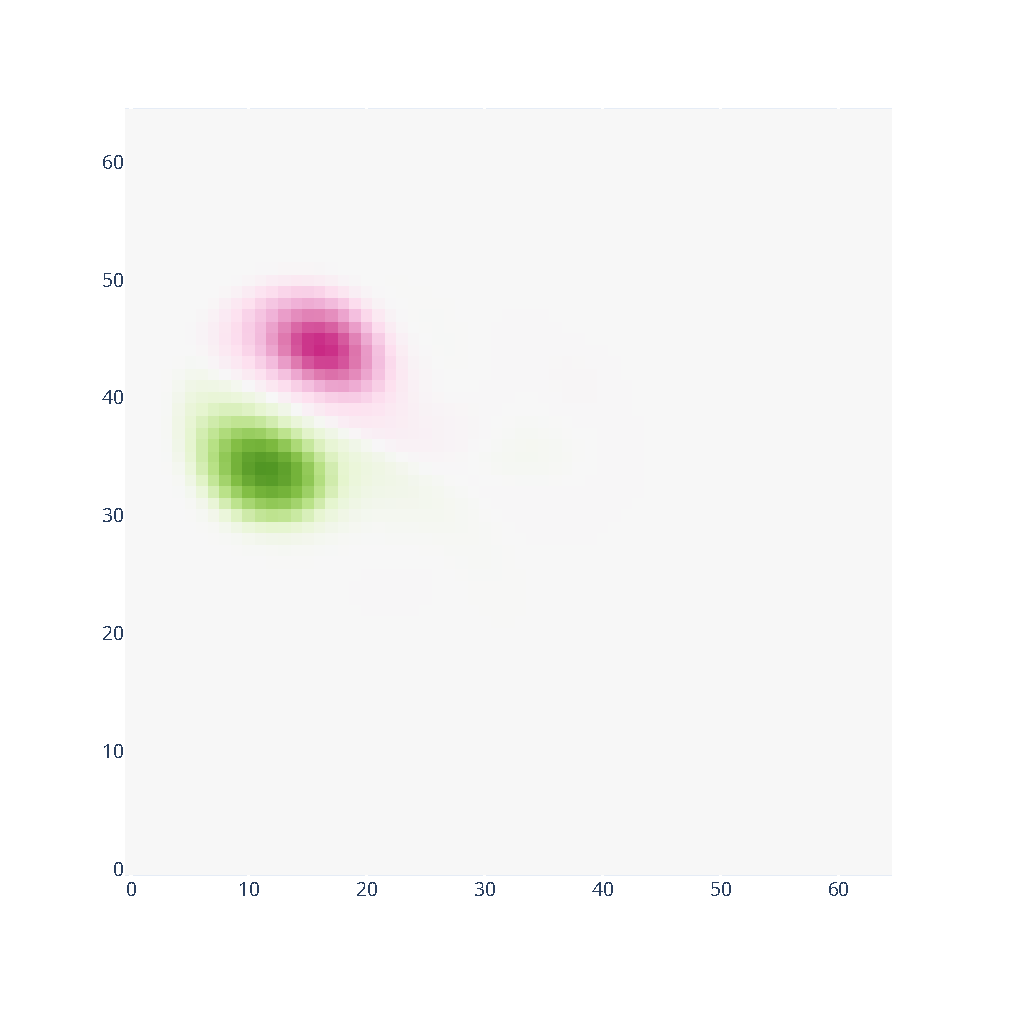
\includegraphics[width=\linewidth]{images/app2d/best_estimate_10.pdf}
	\end{subfigure}
	\hfill
	\begin{subfigure}{0.32\textwidth}
		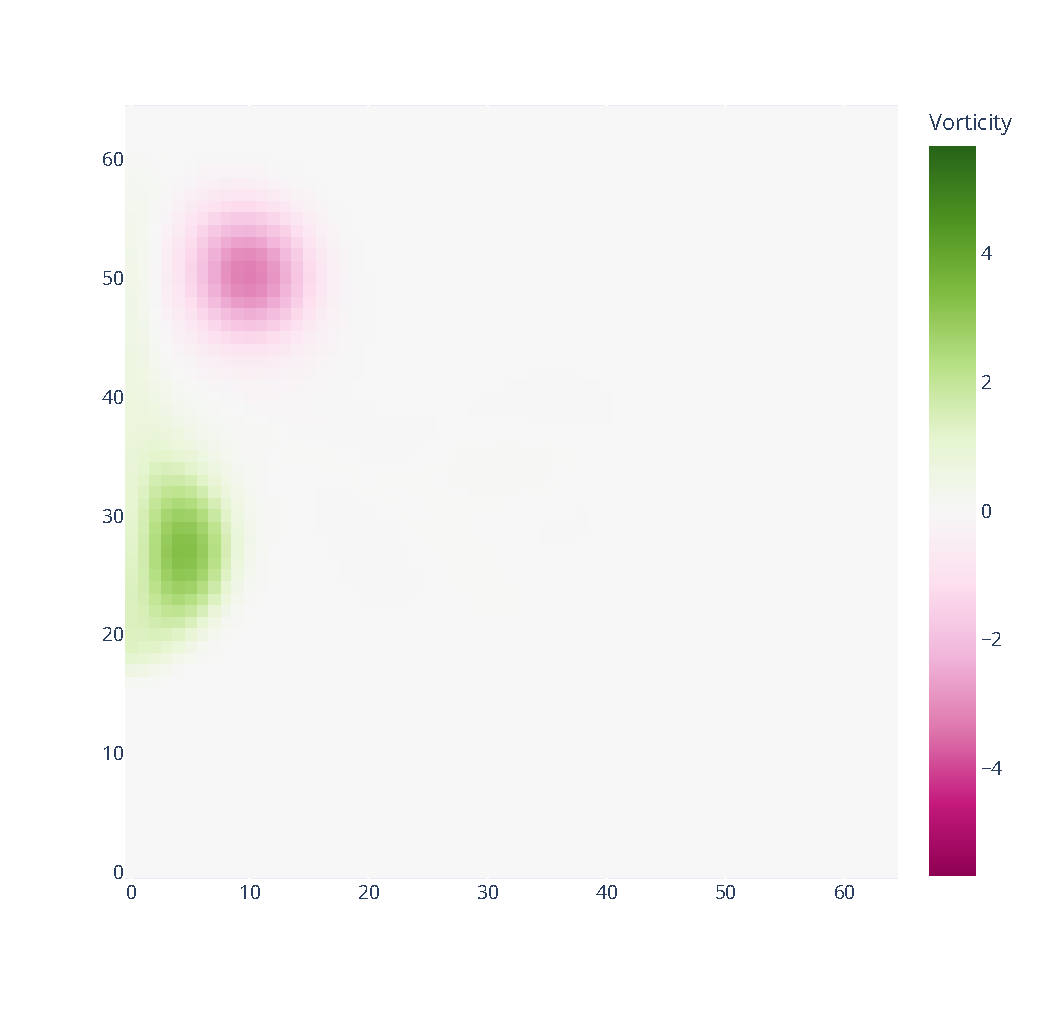
\includegraphics[width=\linewidth]{images/app2d/best_estimate_20.pdf}
	\end{subfigure}
	\caption{Trajectory of the ground truth. The vorticity is represented on a regularly spaced grid. For $t=[1, 5, 10]s.$}
	\label{fig:ref_trajectory}
\end{figure}
Several parameters in the simulation influence the particle distribution and can lead to different results. The first one is the particle size defined by $d_p$. Another significant parameter is $\varepsilon_\omega$, associated with the remeshing process occurring either during the forecast (to prevent high distortion of the particle distribution) or during the Remesh-EnKF filter. $\varepsilon_\omega$ serves as a threshold, determining whether a particle is retained after the remeshing process based on the condition $V_p \Gamma_p > \varepsilon_\omega$. The impact of this parameter is illustrated for one member after the first forward in Figure~\ref{fig:eps_effect}.

\begin{figure}[htbp]
	\centering
	\begin{subfigure}{0.3\textwidth}
		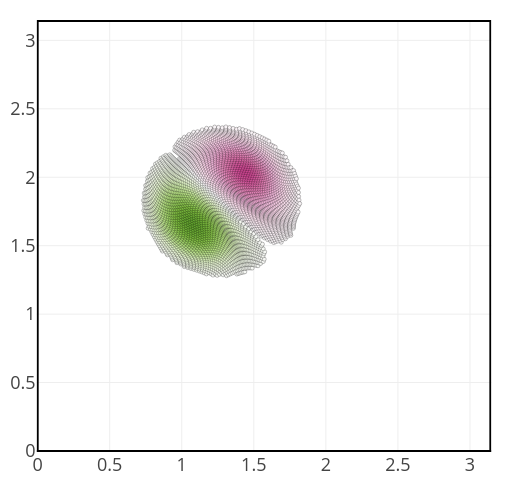
\includegraphics[width=\linewidth]{images/app2d/part_eps_0.1.png}
	\end{subfigure}
	\hfill
	\begin{subfigure}{0.3\textwidth}
		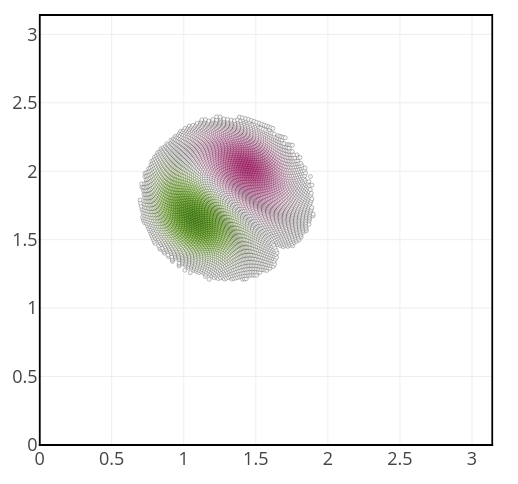
\includegraphics[width=\linewidth]{images/app2d/part_eps_0.01.png}
	\end{subfigure}
	\hfill
	\begin{subfigure}{0.3\textwidth}
		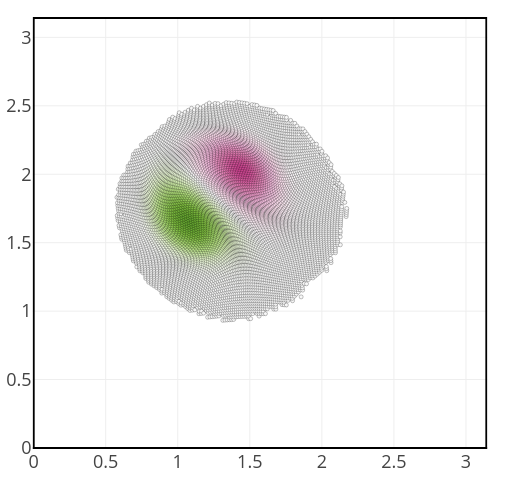
\includegraphics[width=\linewidth]{images/app2d/part_eps_1e-6.png}
	\end{subfigure}
	\caption{Effect of the parameter $\varepsilon_\omega$ on the particle discretization of the solution for one member. From left to right, results for $\varepsilon_\omega = 0.1, 0.01$, and $1.e^{-6}$.}
	\label{fig:eps_effect}
\end{figure}

For the next paragraphs, if the value is not explicitly changed, we use the nominal parameters described in Table \ref{tab:simu_2d} for the simulation.

\subsection{Assimilation parameters and ensemble generation}

\subsubsection{Ensemble distribution}
An ensemble of 32 members is created by sampling distributions over the dipole parameters. We sample the radius $R$, the prescribed velocity $U$, the orientation $\alpha$, and the barycenter $\bm z_{\text{mean}}$. Additionally, the model viscosity $\nu$ is also sampled. All the distributions are summarized in Table \ref{tab:ens_dipole}. The first six members are plotted in Figure \ref{fig:sample_ens}.

\begin{figure}[ht]
	\centering
	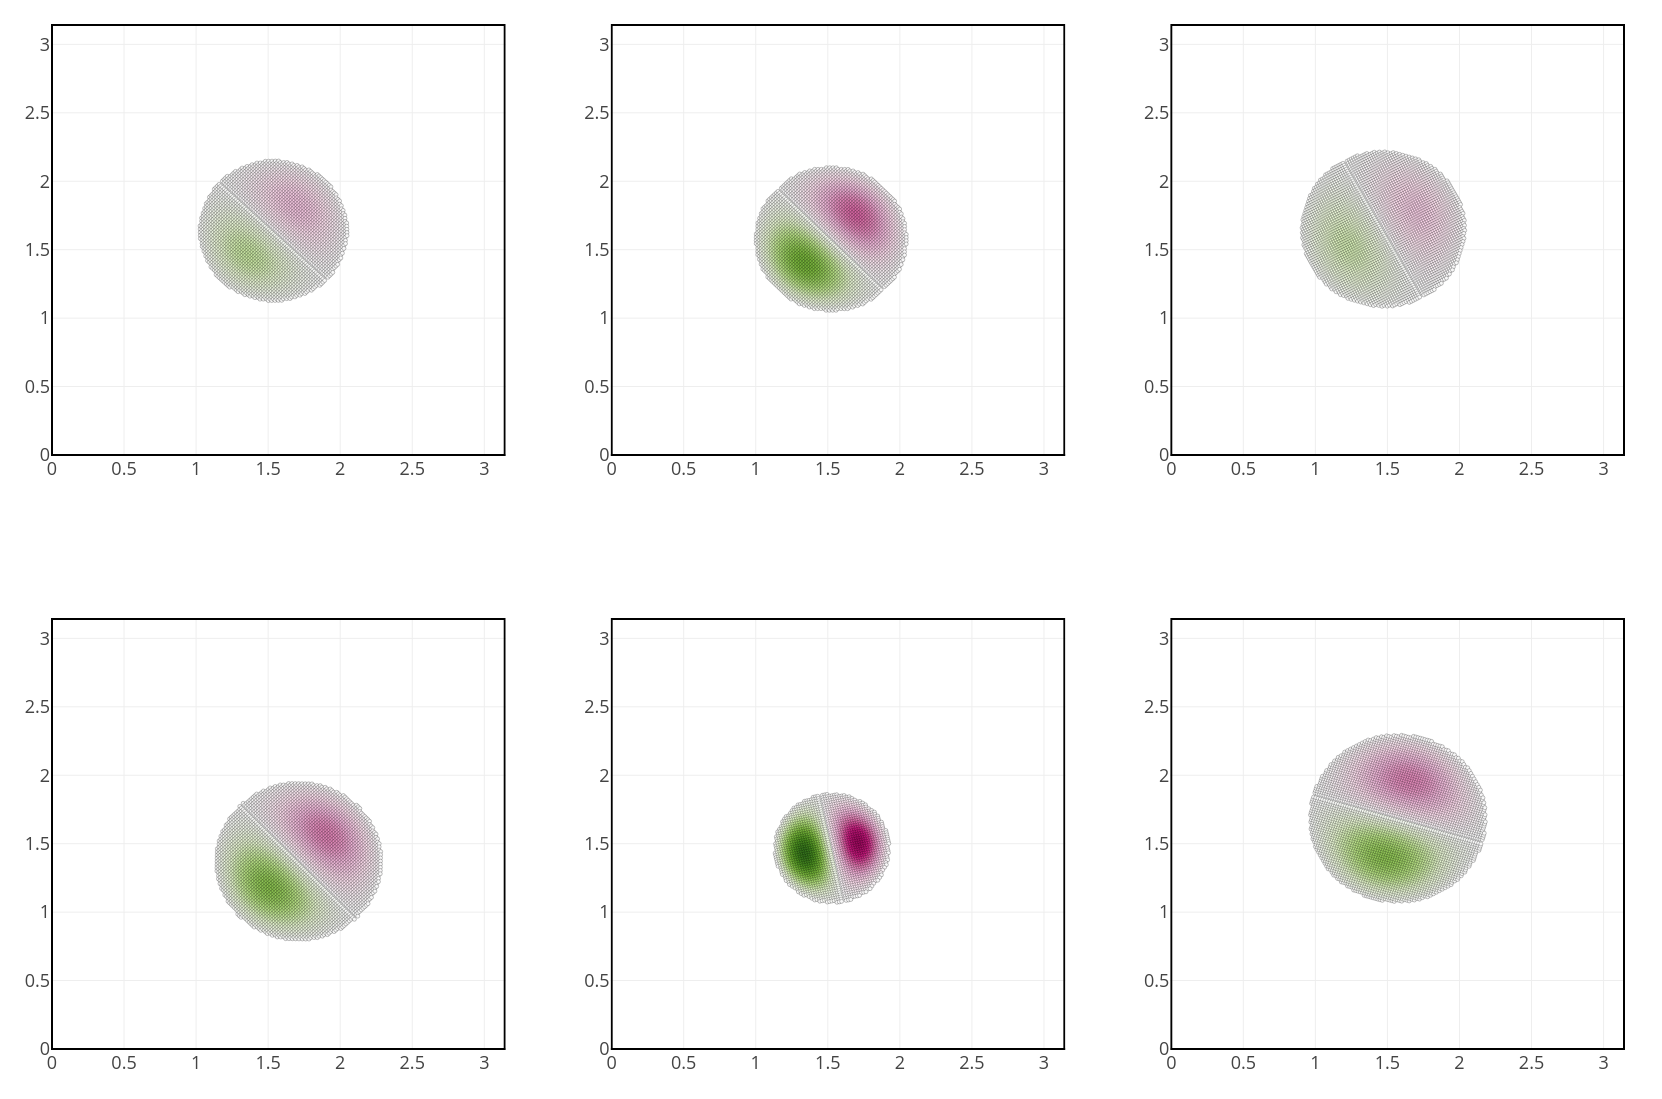
\includegraphics[width=0.9\linewidth]{images/app2d/ensemble_sample.png}
	\caption{Six samples from the initial ensemble.}
	\label{fig:sample_ens}
\end{figure}

The initial vorticity field is first discretized on a regular grid of particles with a characteristic length $d_p$, where each particle receives the circulation $\Gamma_p = \omega(\bm z_p) V_p$, and $V_p = d_p^2$ represents the volume of the particle.

\subsubsection{Error definition}

We use an absolute error absolute \(L_2\)-error defined as $ \frac1\nens \sum_{i = 1}^{\nens} \int_\Omega \left(\omega_i(\z) - \omega^{gt}(\z)\right)^2 \mathrm{d}\z$.
We use the the member error also to evaluate the dispartion of the error estimate.

\subsubsection{Numerical parameters}

The assimilation frequency is defined by the assimilation step $dt_a$. The simulation is performed over a duration of $t_f$. All simulation parameters are summarized in Table \ref{tab:simu_2d}.

Observations are collected on a regular grid of size $N_{\text{obs}}$, measuring both components of the velocity. The observations follow a normal distribution $\mathcal N(0, \sigma_{\text{obs}}^2 \bm{I})$, indicating an ensemble of independent measurements, each characterized by a standard distribution of $\sigma_{\text{obs}}$. An example of observed velocity with and without noise is illustrated in Figure \ref{fig:velocity}.

\begin{figure}[htbp]
	\centering
	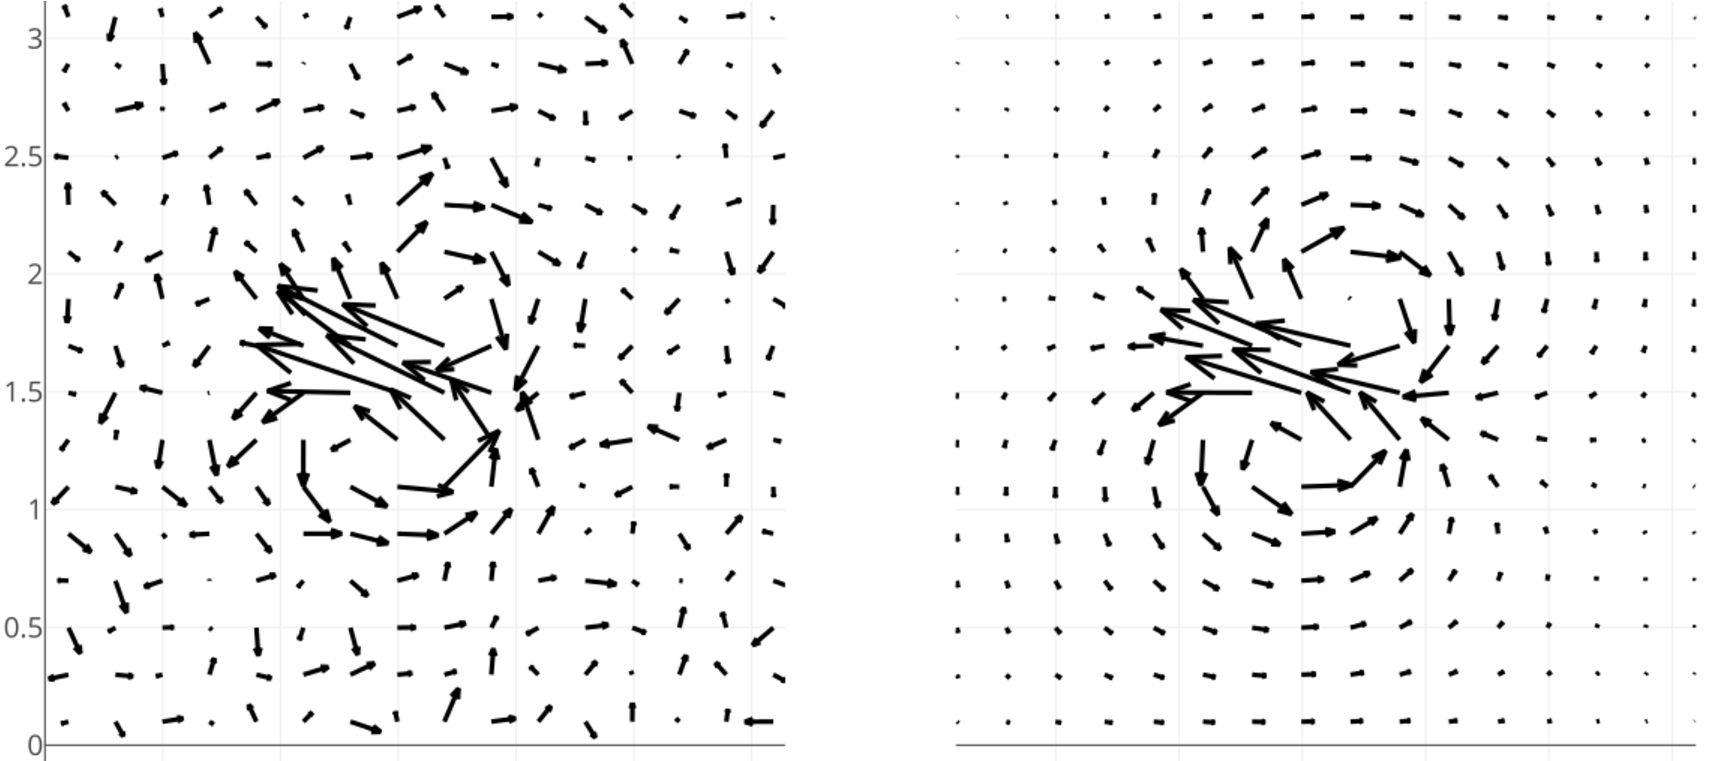
\includegraphics[width=0.8\linewidth]{images/app2d/velocity_ref_recadre.pdf}
	\caption{Observed and reference velocity fields. The error on each component is sample from a centred normal distribution with the nominal value $\sigma_{\text{obs}} = 0.05$.}
	\label{fig:velocity}
\end{figure}

\newpage

\subsection{Results}

\subsubsection{Error through time}

We start by analyzing the assimilation error over time. Figure \ref{fig:assim_time} illustrates the error throughout the assimilation process for the nominal set of assimilation parameters, demonstrating comparable results for both filters. At each assimilation step, the error decrease and avoid the solution to diverge elsewhere.

\begin{figure}[htbp]
	\centering
	\includegraphics*[width=0.7\linewidth]{images/app2d/final/error_in_time.pdf}
	\caption{Error curves through assimilation steps. Left: \(L_2\)-error of the field, Right: Error for the viscosity parameter. With Part-EnKF in blue and Remesh-EnKF in red.}
	\label{fig:assim_time}
\end{figure}

\newpage

\subsubsection{Error with respect to assimilation parameters}
We also assess the performances of the different filters by evaluating the convergence of the error with respect to the assimilation parameters.

We observe the convergence rate concerning data assimilation parameters: The observation precision, which is \(1/\sigma_{\text{obs}}^2\), the number of observations \(N_{\text{obs}}\), the number of assimilation step \(N_{\text{assim}}\).

The Figure \ref{fig:obs_precision_1} illustrate a decreasing error bias and variances with respect to observation precision similarly for both filter.What is striking in the same Figure~\ref{fig:obs_precision_2} but in the log-scale is the regular convergence rate for both filter with respect to the observation precision. The order of convergence is about 0.68 for Part-EnKF and 0.75 for Remesh-EnKF.

\begin{figure}[h!]
	\centering
	\begin{subfigure}{0.49\linewidth}
		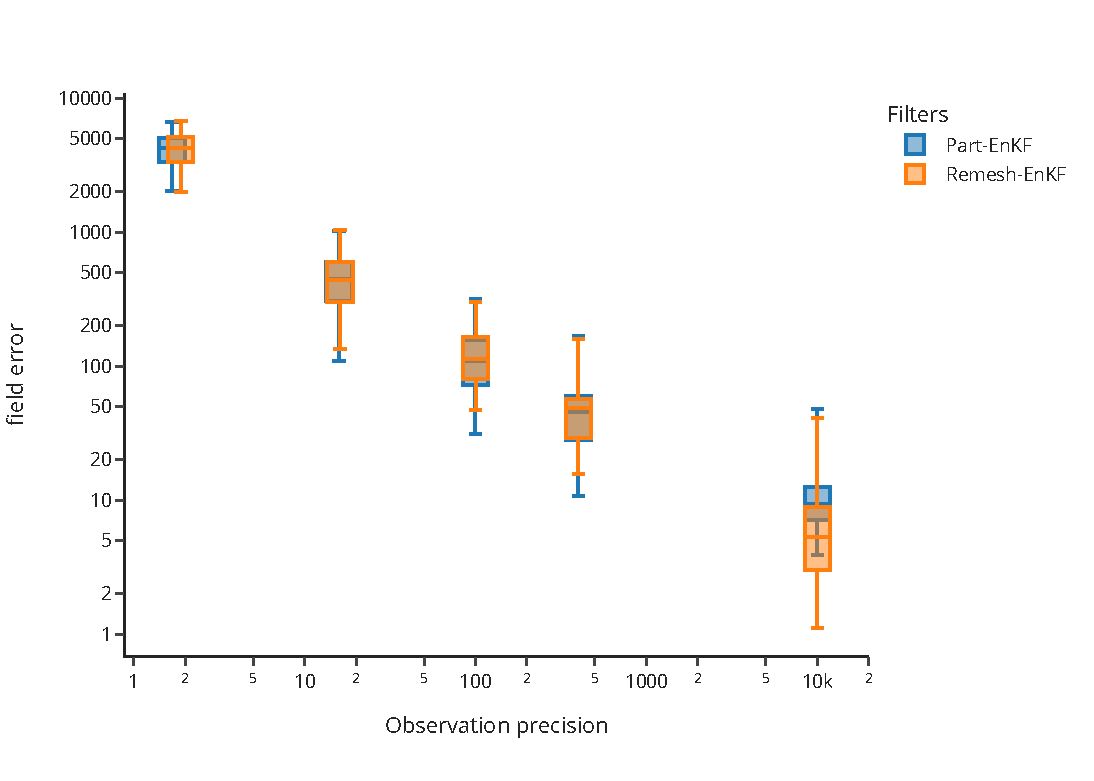
\includegraphics[width=\linewidth]{./images/app2d/final/MSE_obs_precision_box.pdf}
		\caption{}
		\label{fig:obs_precision_1}
	\end{subfigure}
	\begin{subfigure}{0.49\linewidth}
		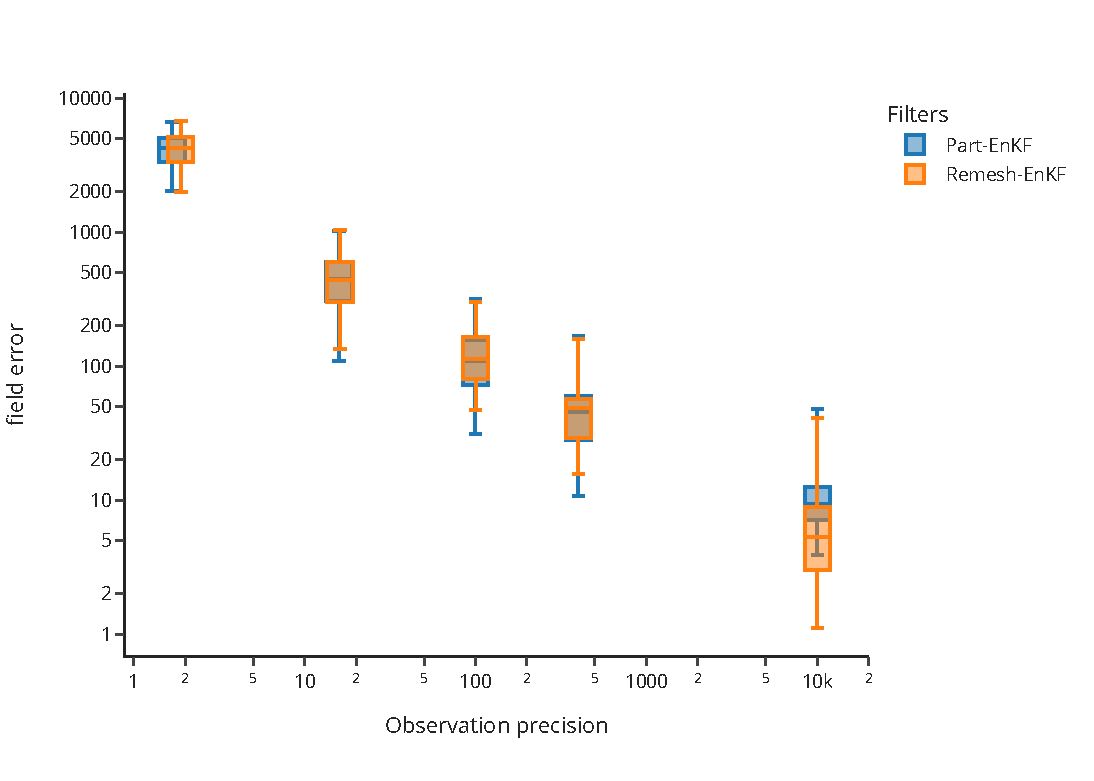
\includegraphics[width=\linewidth]{./images/app2d/final/MSE_obs_precision_box_log.pdf}
		\caption{}
		\label{fig:obs_precision_2}
	\end{subfigure}
	\caption{Box plots of the state error w.r.t. $1/\sigma_{\text{obs}}^2$.}
\end{figure}


In the Figure~\ref{fig:na_1} the reduction of error is still prominent and show a reduction of variance as the number of observation increase. In the log-scale Figure~\ref{fig:na_2}, the error decrease also at a constant rate for both Filter. We notice, we notice a stronger order of 1.8 for the Remesh-EnKF compared to an order of 1.4 for Part-EnKF.

\begin{figure}[h!]
	\centering
	\begin{subfigure}{0.49\linewidth}
		\centering
		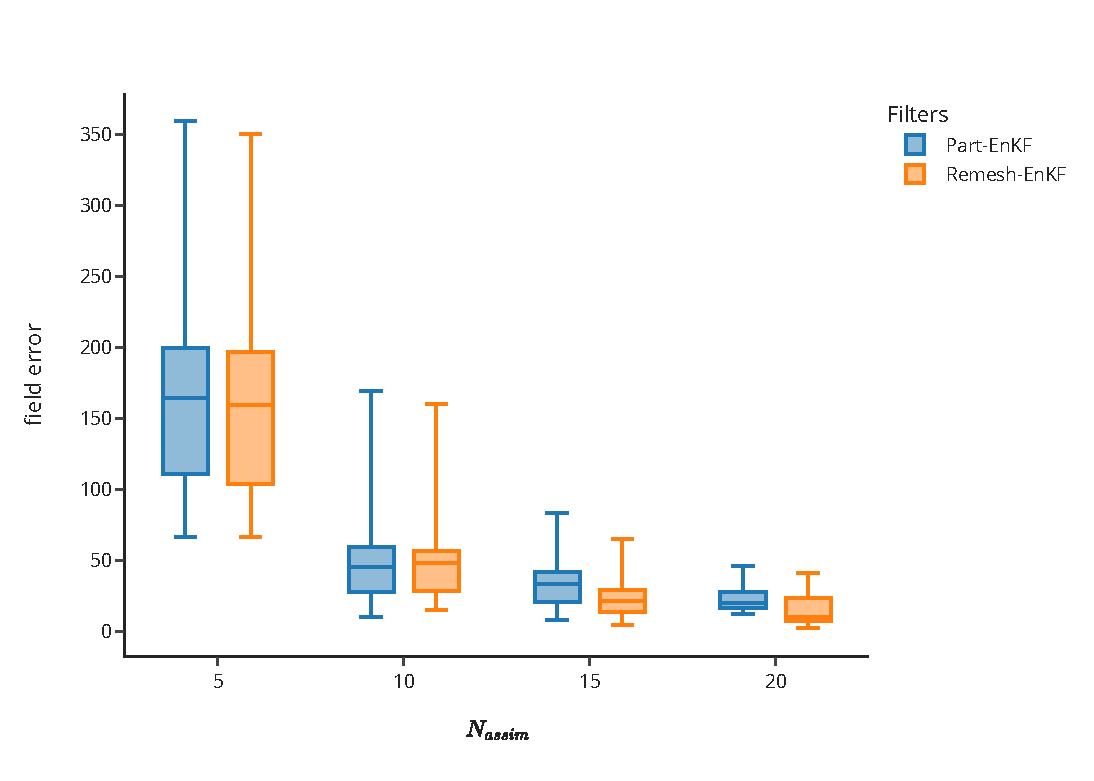
\includegraphics[width=\linewidth]{./images/app2d/final/MSE_na_box.pdf}
		\caption{}
		\label{fig:na_1}

	\end{subfigure}
	\begin{subfigure}{0.49\linewidth}
		\centering
		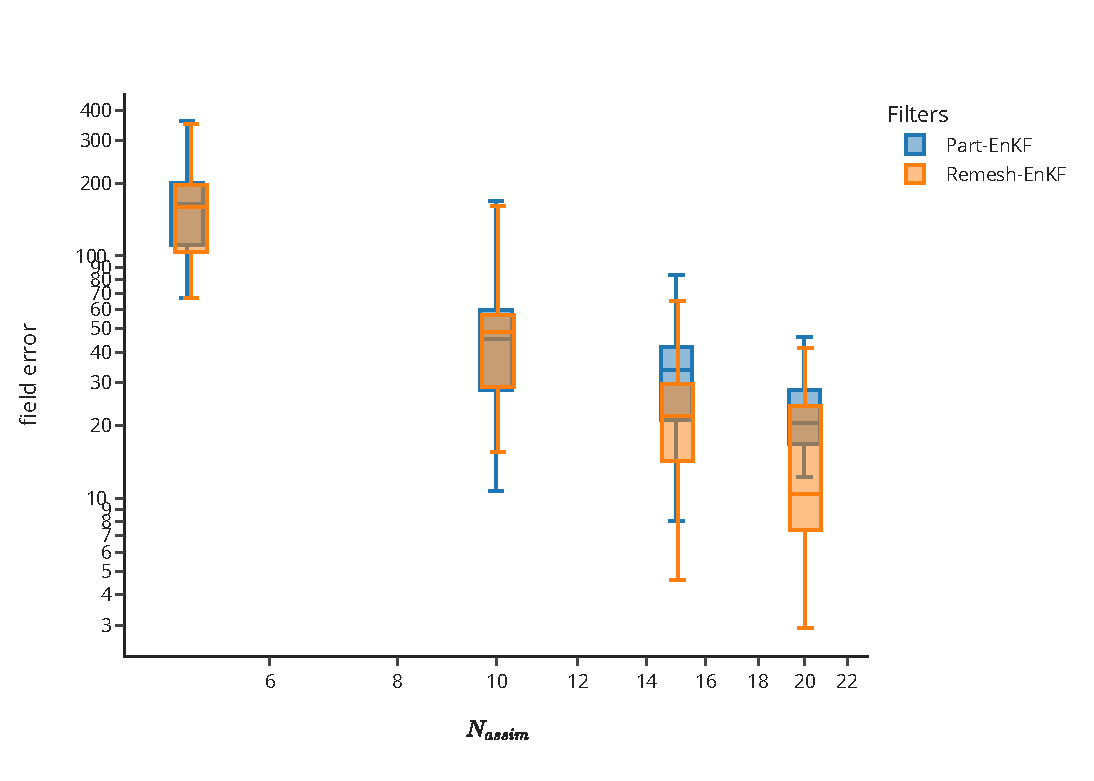
\includegraphics[width=\linewidth]{./images/app2d/final/MSE_na_box_log_log.pdf}
		\caption{}
		\label{fig:na_2}
	\end{subfigure}
	\caption{Box plots of the state error w.r.t. $N_{\text{assim}}$.}
	\label{fig:na}

\end{figure}

Finally, we analyse the error convergence with respect to the number of observation. Observation location increase regularly in both axis. In Figure~\ref{fig:nobs_1}, the error estimate decrease but

\begin{figure}[h!]
	\centering
	\begin{subfigure}{0.49\linewidth}
		\centering
		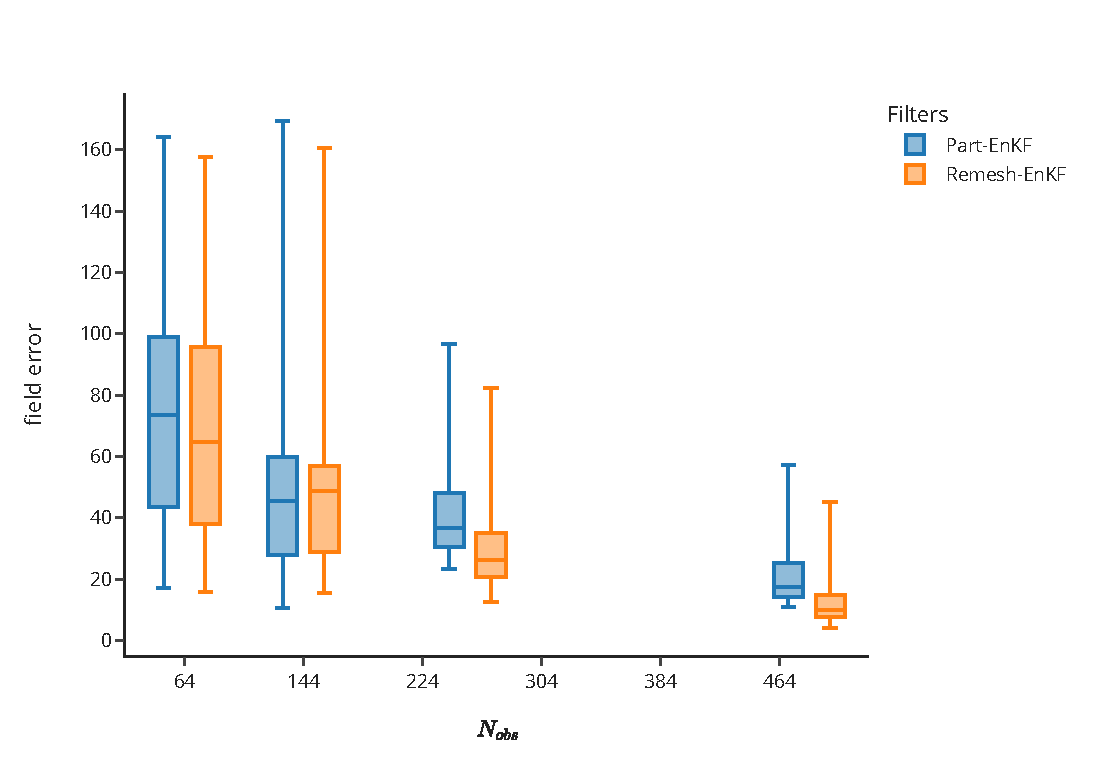
\includegraphics[width=\linewidth]{./images/app2d/final/MSE_nobs_box.pdf}
		\caption{Box plots of the state error w.r.t. $N_{\text{obs}}$.}
		\label{fig:nobs_1}
	\end{subfigure}
	\begin{subfigure}{0.49\linewidth}
		\centering
		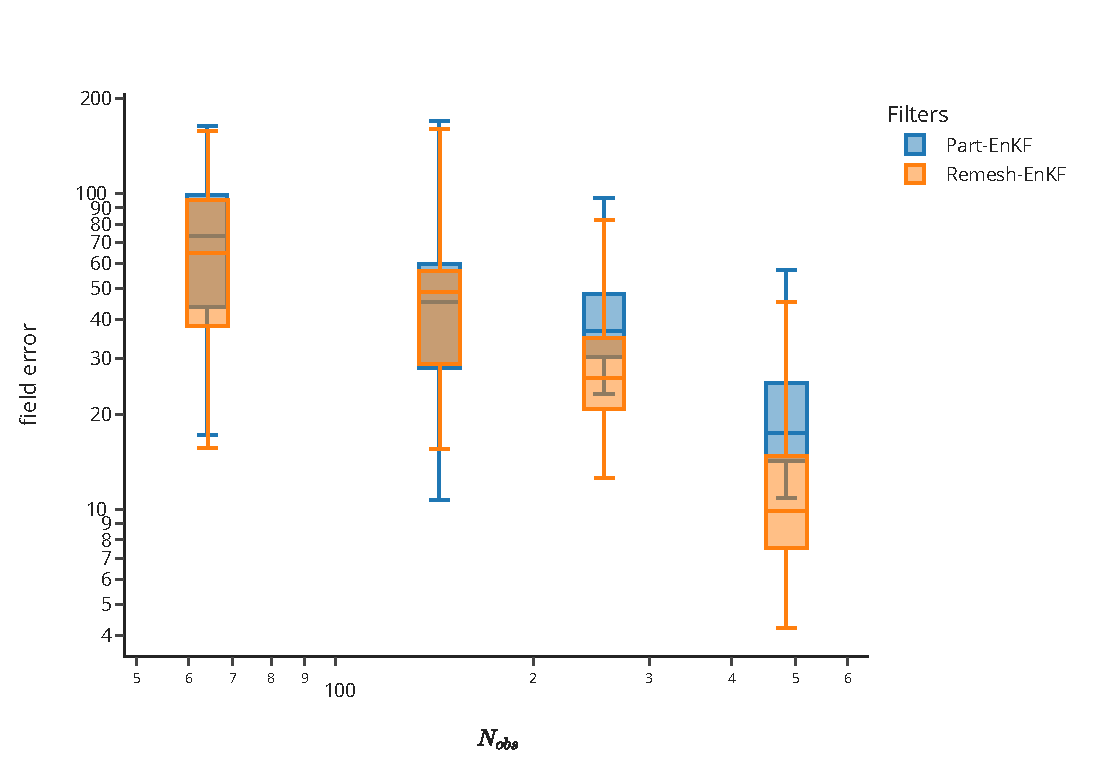
\includegraphics[width=\linewidth]{./images/app2d/final/MSE_nobs_box_log_log.pdf}
		\caption{Box plots of the state error w.r.t. $N_{\text{obs}}$.}
		\label{fig:nobs_2}
	\end{subfigure}
	\label{fig:nobs}

	\label{fig:assim_params}
\end{figure}

\subsubsection{Error with respect to simulation parameters}

To better understand the differences, we also evaluate the evolution of the error with respect to particle discretization parameters. For the Part-EnKF, remember that each member has its own particle discretization that flows according to the dipole direction and velocity. Each analyzed member's solutions are then respectively projected on their member discretization. However, this scheme could introduce different sources of error. First, due to particle irregularity in the particle distribution, it introduced severe approximation that led to errors between the analyzed and the approximated solution. Even more seriously, certain parts of the solution may vanish as no particle in the support can interpolate it. This effect could be appreciated on several samples of the ensemble where the analysis is projected on a non-conforming particle discretization. For instance, we analyzed the first assimilation step of one member for the different filters. If the analyzed field is known over the space domain, we observed in Figure~\ref{fig:assim_member} that the Remesh-Filter and Part-Grid-EnKF are only able to interpolate the entire solution. The Part-EnKF is not entirely able to interpolate the solution with the forecast member discretization.
Moreover, some distortions observed in the particle distribution are not in line with the analyzed field flow. These remarks are more critical when the forecast step is longer, leading to high errors, or when the size of the support is lower. Moreover, the approximation of Section \ref{regressionOperator} will introduce the approximation error function of the size of the particles. For instance, the particle will not conserve the total circulation due to a quadrature error, which is the opposite case for the Remesh-EnKF filter.

\begin{figure}[h!]
	\centering
	\begin{subfigure}{0.45\textwidth}
		\centering
		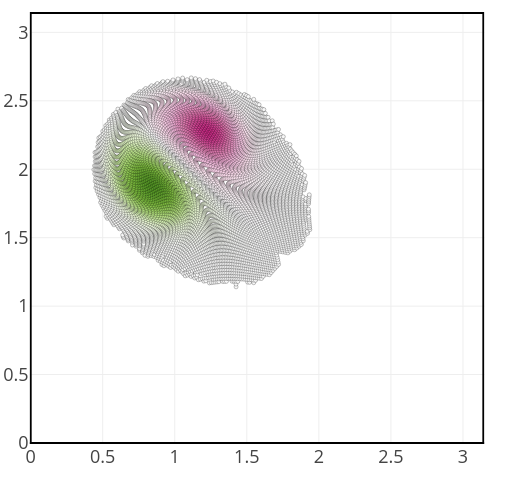
\includegraphics[width=0.8\linewidth]{./images/app2d/assim_member_forecast.png}
	\end{subfigure}
	% \hfill
	\begin{subfigure}{0.45\textwidth}
		\centering
		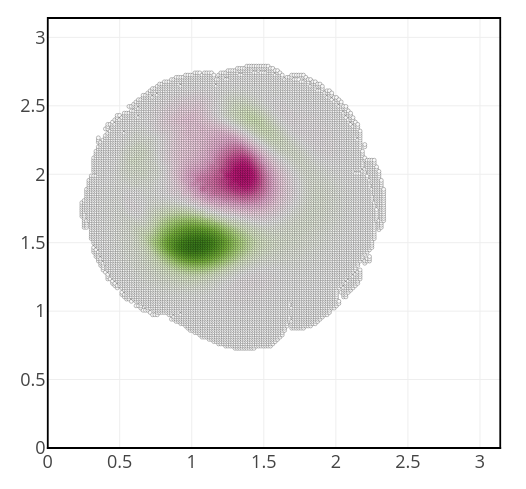
\includegraphics[width=0.8\linewidth]{./images/app2d/assim_member_rmf.png}
	\end{subfigure}
	\begin{subfigure}{0.45\textwidth}
		\centering
		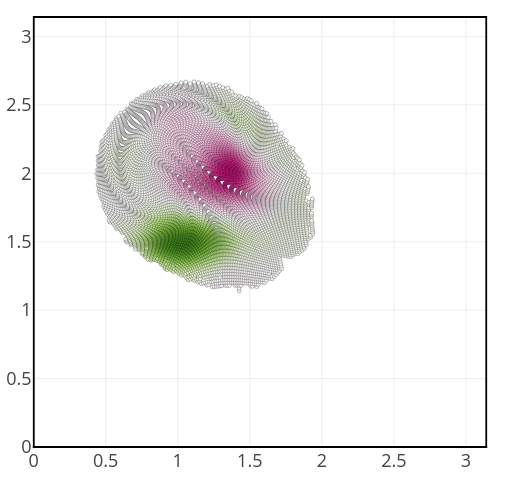
\includegraphics[width=0.8\linewidth]{./images/app2d/assim_member_ppf.png}
	\end{subfigure}
	% \hfill
	\begin{subfigure}{0.45\textwidth}
		\centering
		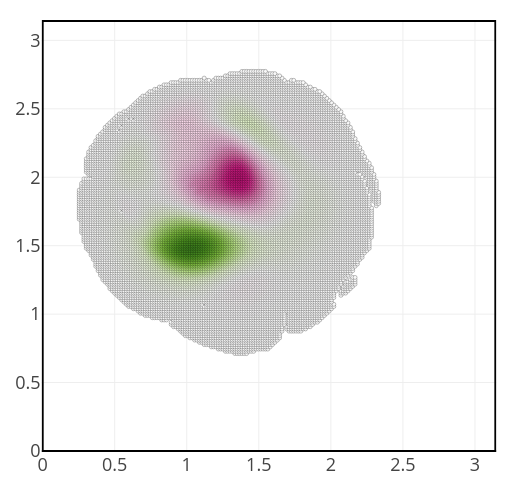
\includegraphics[width=0.8\linewidth]{./images/app2d/assim_member_pgf.png}
	\end{subfigure}
	\caption{Assimilation of one member with a forecast discretization unadapted to the analyses solution. From left to right and up to down: the forecast member, the analyses member with the Remesh-EnKF filter, the analyses member with the Part-EnKF filter and finally the analyses member with the Part-Grid-EnKF. The forecast discretization use by the Part-EnKF is not always a well support of approximation for the analyses and introduce discretization errors.}
	\label{fig:assim_member}
\end{figure}

To evaluate the effect of the size of the support, we varied the value of $\epsilon_{\omega}$. We have seen in Figure~\ref{fig:eps_effect} that this parameter affects the number of particles and, thus, the size of the support. We observe relatively poor difference between the different value. However, the error stabilizes rapidly by decreasing the threshold. A relatively low effect is also observed on the Remesh-EnKF due to truncation errors at the border of the dipole solution.

Thanks to the Part-Grid-EnKF, we could better decompose the error. On the one hand, the difference between the Part-EnKF and the Part-Grid-EnKF is linked to the support and the distortion of the particle distribution. On the other hand, the remaining difference between Part-Grid-EnKF is due to the particle approximation error. This hypothesis is confirmed by analyzing the error with respect to the particle size $d_p$ in Figure \ref{fig:simu_parameters_error}. We observe that the error for Part-EnKF and Part-Grid-EnKF increases proportionally with $d_p$ as for the approximation error. The same order of magnitude for the different filters is observed is observed for relatively small particle sizes. This confirmed the high effect of the particle approximation in this case. Using a regression operator to approximate the analyzed solution should alleviate this effect provided other particle discretization considerations (distortion, support size) as illustrated in Part~\ref{App_1D} and the choice of an adequate penalty coefficient to succeed in approximating the solution.

\begin{figure}[htbp]
	\centering

	\begin{subfigure}{0.48\textwidth}
		\centering
		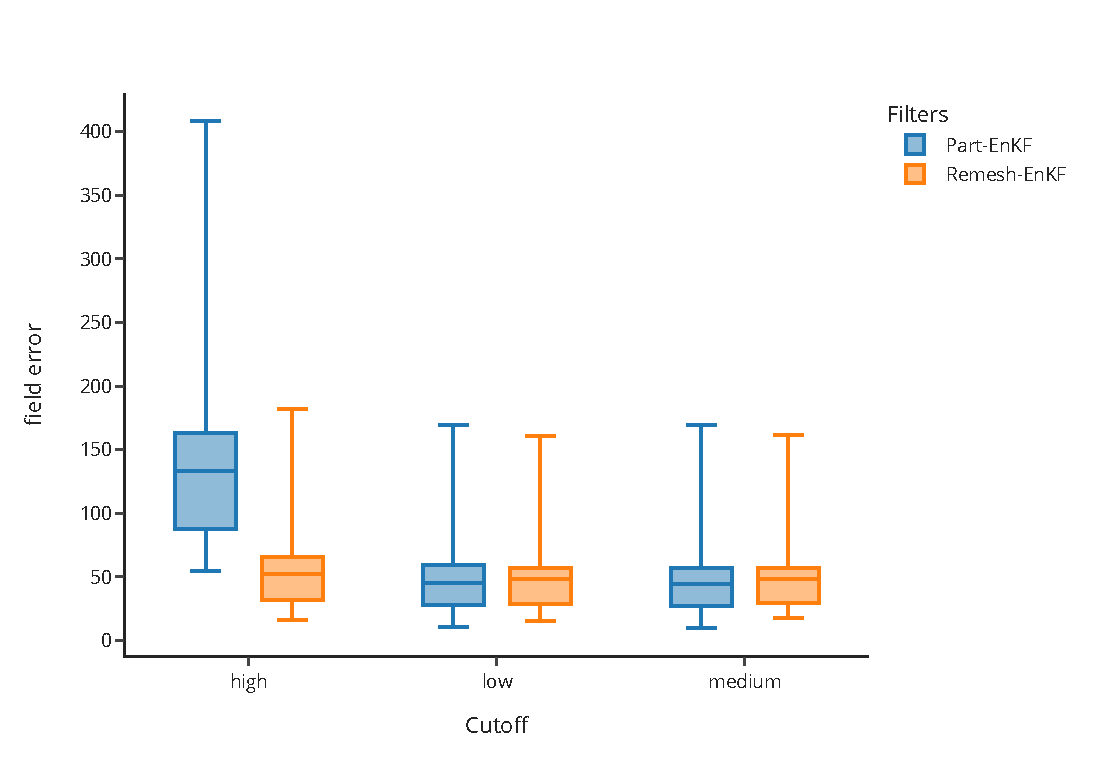
\includegraphics[width=\linewidth]{./images/app2d/final/MSE_cutoff_box.pdf}
		\captionsetup{labelformat=empty}
		\caption{state error w.r.t. $\varepsilon_{\omega}$}
		\label{fig:eps_omega}
	\end{subfigure}
	\hfill
	\begin{subfigure}{0.48\textwidth}
		\centering
		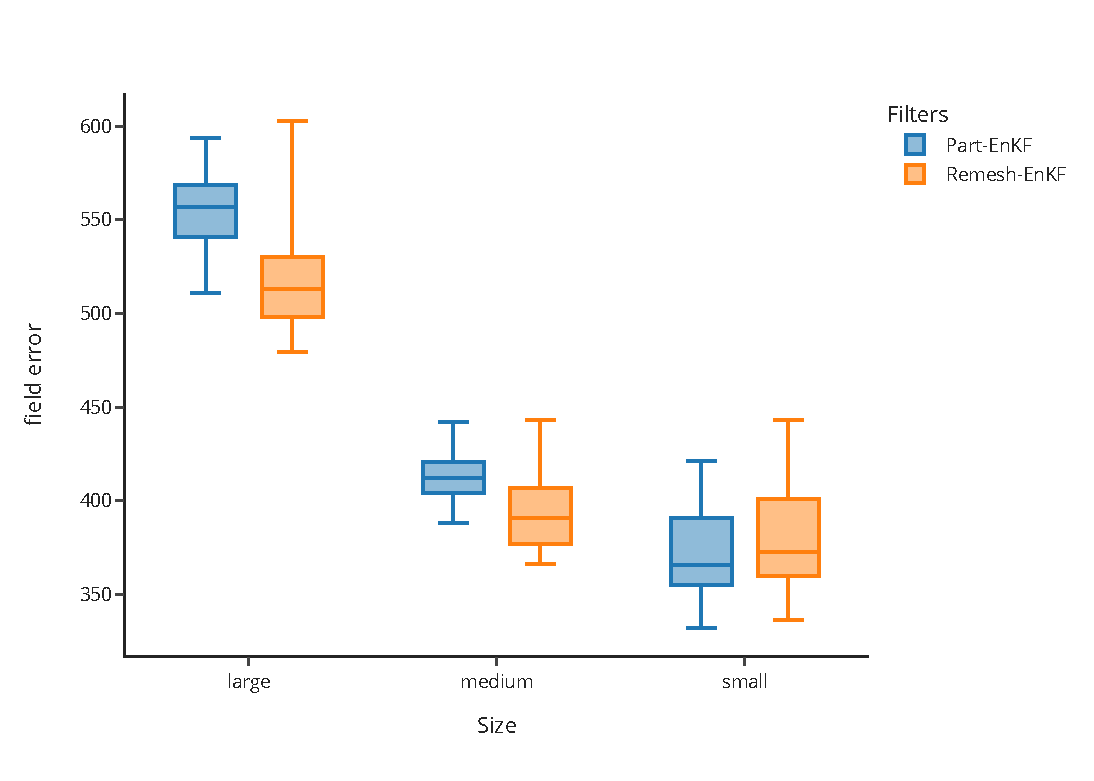
\includegraphics[width=\linewidth]{./images/app2d/final/MSE_size_box.pdf}
		\captionsetup{labelformat=empty}
		\caption{state error w.r.t. $d_p$}
		\label{fig:np_visc}
	\end{subfigure}

	\caption{Error box plots for simulation parameters. The effect of $\varepsilon_{\omega}$ on the error is particularly observed on high value. The Part-EnKF error is strongly linked to $d_p$ through the particle approximation error.}
	\label{fig:simu_parameters_error}
\end{figure}

This discussion pointed out the high dependency of the Part-EnKF on particle discretization. As it could be understood, the particle discretization of a member could be too far from the solution support of particles. This opens the question of the choice of particle discretization. As suggested in Part~\ref{App_1D}, an error estimation could be introduced to choose between the different filters. On the other hand, other approaches could be to select the member with the maximum likelihood estimate to approximate the solution. This proposition has to be evaluated because it could considerably reduce the variance of the ensemble. Moreover, we note that the particle approximation could rapidly have a high effect, as seen in this Part.

\newpage
%We have seen the importance of the support size for the Part-EnKF filter...

